\documentclass{vldb}
\usepackage{graphicx}
\usepackage{balance}  % for  \balance command ON LAST PAGE  (only there!)
\usepackage{enumitem}
\usepackage{times}
\usepackage{subfigure}
\let\proof\relax
\let\endproof\relax
\usepackage{amsmath,amssymb,amsthm}
\usepackage{graphicx,color}
\usepackage{verbatim}
\usepackage{framed}
\usepackage[ruled,vlined]{algorithm2e}
\usepackage{framed}
\usepackage[normalem]{ulem}
\usepackage[export]{adjustbox}


\usepackage[font={small,it}]{caption}

\renewcommand{\baselinestretch}{1.0}

\renewcommand*\ttdefault{cmvtt}
\usepackage[T1]{fontenc}

% \usepackage{floatrow}
% \floatsetup[table]{font=scriptsize}
% \renewcommand\FBbskip{-10pt}


\newtheorem*{theorem*}{Theorem}
\newtheorem{theorem}{Theorem}
\newtheorem*{lemma*}{Lemma}
\newtheorem{lemma}{Lemma}
\newtheorem{definition}{Definition}
\newtheorem{example}[definition]{Example}
\newcounter{prob}
\newtheorem{problem}[prob]{Problem}

\newcommand{\agp}[1]{\textcolor{green}{Aditya: #1}}
\newcommand{\mrj}[1]{\textcolor{red}{#1}}
\newcommand{\mrjdel}[1]{\textcolor{red}{\sout{#1}}}

\newcommand{\squishlist}{
   \begin{list}{$\bullet$}
    { \setlength{\itemsep}{0pt}
      \setlength{\parsep}{2pt}
      \setlength{\topsep}{2pt}
      \setlength{\partopsep}{0pt}
    }
}
\newcommand{\stitle}[1]{\vspace{0.5em}\noindent\textbf{#1}}
\newcommand{\squishend}{\end{list}}
\newcommand{\eat}[1]{}
\newcommand{\papertext}[1]{#1}
\newcommand{\techreporttext}[1]{}


\newcommand{\calD}{\mathcal{D}\xspace}


\newenvironment{denselist}{
    \begin{list}{\small{$\bullet$}}%
    {\setlength{\itemsep}{0ex} \setlength{\topsep}{0ex}
    \setlength{\parsep}{0pt} \setlength{\itemindent}{0pt}
    \setlength{\leftmargin}{1.5em}
    \setlength{\partopsep}{0pt}}}%
    {\end{list}}

\makeatletter
\def\@copyrightspace{\relax}
\makeatother

\begin{document}

\title{Demo: Smart Drill-Down}
\numberofauthors{3} 
\author{
\alignauthor
Manas Joglekar\\
       \affaddr{Stanford University}\\
%       \affaddr{353 Serra Mall}\\
%	   \affaddr{Stanford, California 94305}\\
       \email{manasrj@stanford.edu}
\alignauthor
Hector Garcia-Molina\\
       \affaddr{Stanford University}\\
%       \affaddr{353 Serra Mall}\\
%	   \affaddr{Stanford, California 94305}\\
       \email{hector@cs.stanford.edu}
\alignauthor 
Aditya Parameswaran\\
       \affaddr{University of Illinois (UIUC)}\\
%       \affaddr{Champaign, Illinois 61820}\\
       \email{adityagp@illinois.edu}
}
\maketitle

\begin{abstract}
We present a data exploration system equipped with {\em smart drill-down},
a novel operator for interactively exploring a relational table
to discover and summarize ``interesting'' groups of tuples.
The summary consists of a set of {\em rules}, where each rule describes a group of tuples.
For instance, the rule $(a, b, \star, 1000)$ tells us that
there are a thousand tuples with value $a$ in the first column and $b$
in the second column (and any value in the third column).
Smart drill-down presents an analyst with a list of rules that
together describe interesting aspects of the table.
The analyst can tailor the definition of interesting,
and can interactively apply smart drill-down on an existing rule to
explore that part of the table. The problems underlying smart drill-down are {\sc NP-Hard}, so our system uses an approximation algorithm for choosing the best list of rules to display. In addition, our system uses a dynamic sampling and memory management scheme to achieve low response times while interacting with large tables.
\end{abstract}

%!TEX root = TableSummarizationDemo.tex


\section{Introduction} \label{sec:intro} 

Analysts often use OLAP (Online Analytical Processing) operations
such as drill down~\cite{export:69578} to explore
relational databases. 
These operations are very useful for analytics and data exploration and have stood the test of time;
all commercial OLAP systems 
in existence support these operations. (Recent reports estimate the size of the OLAP market to be \$10+ Billion~\cite{gartner}.)

But there are several cases where drill down is ineffective; 
for instance, when the column being drilled down on has a large number of distinct values,
the results can easily overwhelm analysts by presenting them with too many 
values. Furthermore, drill down only allows us to explore one column at a time, instead of allowing simultaneous drill downs
on multiple columns---moreover, simultaneously drilling down on multiple columns 
is likely to again suffer from the problem
of having too many results, due to having too many distinct combinations of column values.

In this demonstration, we present a new interaction operator called {\em smart drill down}, 
that is an extension to a traditional 
drill down operator, aimed at providing {\em complementary}
functionality to drill down in cases where drill down is
ineffective. Smart drill down makes it possible for analysts to zoom into
the more ``interesting'' parts of a table or a database,
with fewer operations, and without having to examine as much
data as traditional drill down.
Note that our goal is {\em not} to replace traditional 
drill down functionality, which we believe is fundamental;
instead, our goal is to provide auxiliary functionality 
which analysts are free to use whenever they find 
traditional drill downs ineffective.

In addition to this new operator called smart drill down, our system implements novel sampling techniques to compute the results for this
operator {\em in an interactive fashion} on increasingly larger databases. 
Unlike the traditional OLAP setting, these computations 
require no pre-materialization, and can be implemented 
within or on top of any relational database system.

The best way to explain smart drill down is through a simple example.

\begin{example}\label{ex:introexample}
Consider a table with columns `Department Store', `Product', `Region'
and `Sales'. Suppose an analyst queries for tuples
where Sales were higher than some threshold, in order
to find the best selling products.
If the resulting table has many tuples,
the analyst can use traditional drill down to explore it.
For instance, the system may initially tell the analyst there are
6000 tuples in the answer, represented by the tuple ($\star$, $\star$, $\star$, $6000$, $0$),
as shown in Table~\ref{table:introexample0}.
The $\star$ character is a wildcard that matches any value in the database.
The Count attribute can be replaced by a Sum aggregate over some measure column,
e.g., the total sales.
The right-most Weight attribute is the number of non-$\star$ attributes; 
its significance will be discussed shortly.
If the analyst drills down on the Store attribute (first $\star$),
then the operator displays all tuples of the form ($X$, $\star$, $\star$, $C$, $1$),
where $X$ is a Store in the answer table, and $C$
is the number of tuples for $X$ (or the aggregate sales for $X$).

Instead, when the analyst uses smart drill down on Table~\ref{table:introexample0},
he obtains Table~\ref{table:introexample}.
The ($\star$, $\star$, $\star$, $6000$) tuple is expanded into $3$ tuples
that display noteworthy or interesting drill downs.
The number $3$ is a user specified parameter, which we call $k$.

For example, the tuple (Target, bicycles, $\star$, $200$, $2$)
says that there are $200$ tuples (out of the 6000) with
Target as the first column value and bicycle as the second.
This fact tells the analyst that Target is selling a lot of bicycles.
The next tuple tells the analyst that comforters are selling well in
the MA-3 region, across multiple stores. The last tuple
states that Walmart is doing well in general over multiple products and regions.
We call each tuple in Table~\ref{table:introexample} a {\em rule}
to distinguish it from the tuples in the original table that is being explored.
Each rule summarizes the set of tuples that are described by it.
Again, instead of Count, the operator can display a Sum aggregate, such as
the total Sales.

\begin{table}
\scriptsize
\centering
\begin{tabular}{| l | l | l | l | l |}
\hline Store & Product & Region & Count & Weight \\
\hline
$\star$ & $\star$ & $\star$ & $6000$ & $0$ \\ \hline
\end{tabular}
\vspace{-10pt}
\caption{Initial summary}\label{table:introexample0}
\vspace{-5pt}
\end{table}

\begin{table}
\scriptsize
\centering
\begin{tabular}{| l | l | l | l | l |}
\hline Store & Product & Region & Count & Weight \\
\hline
$\star$ & $\star$ & $\star$ & $6000$ & $0$ \\ \hline
$\triangleright$ Target & bicycles & $\star$ & $200$ & $2$ \\ \hline
$\triangleright$ $\star$ & comforters & MA-3 & $600$ & $2$ \\ \hline
$\triangleright$ Walmart & $\star$ & $\star$ & $1000$ & $1$ \\ \hline
\end{tabular}
\vspace{-10pt}
\caption{Result after first smart drill down}\label{table:introexample}
\vspace{-10pt}
\end{table}

\begin{table}
\scriptsize
\centering
\vspace{-5pt}
\begin{tabular}{| l | l | l | l | l |}
\hline Store & Product & Region & Count & Weight \\
\hline
$\star$ & $\star$ & $\star$ & $6000$ & $0$ \\  \cline{1-5}
$\triangleright$ Target & bicycles & $\star$ & $200$ & $2$ \\ \cline{1-5}
$\triangleright$ $\star$ & comforters & MA-3 & $600$ & $2$ \\ \cline{1-5}
$\triangleright$ Walmart & $\star$ & $\star$ & $1000$ & $1$ \\ \cline{2-5}
$\triangleright$ $\triangleright$ Walmart & cookies & $\star$ & $200$ & $2$ \\ \cline{2-5}
$\triangleright$ $\triangleright$ Walmart & $\star$ & CA-1 & $150$ & $2$ \\ \cline{2-5}
$\triangleright$ $\triangleright$ Walmart & $\star$ & WA-5 & $130$ & $2$ \\ \hline
\end{tabular}
\vspace{-10pt}
\caption{Result after second smart drill down} \label{table:introexample2}
\vspace{-10pt}
\end{table}

Say that after seeing the results of Table~\ref{table:introexample},
the analyst wishes to dig deeper into the Walmart tuples
represented by the last rule.
For instance, the analyst may want to know
which states Walmart has more sales in, or which products they sell
the most. In this case, the analyst clicks on the Walmart rule,
obtaining the expanded summary in Table~\ref{table:introexample2}.
The three new rules in this table provide additional information
about the $1000$ Walmart tuples.
In particular, one of the new rules shows that
Walmart sells a lot of cookies; the others show it sells a lot of products in
the regions CA-1 and WA-5.

When the analyst clicks on a rule $r$, smart drill down
expands $r$ into $k$ sub-rules that as a set are deemed to be ``interesting.''
There are three factors that make a rule set interesting.
One is if it contains rules with high Count (or total sales) fields,
since the larger the count, the more tuples are summarized.
A second factor is if the rules have high weight (number of non-$\star$ attributes).
For instance, the rule (Walmart, cookies, AK-1, $200$, $3$)
seems more interesting than (Walmart, cookies, $*$, $200$, $2$)
since the former tells us the high sales are concentrated in a single region.
A third desirability factor is diversity:
For example, if we already have the rule (Walmart, $\star$, $\star$, $1000$, $1$)
in our set, we would rather have the rule (Target, bicycles, $\star$, $200$, $2$)
than (Walmart, bicycles, $\star$, $200$, $2$) since the former rule
describes tuples that are not described by the first rule.

Our system combines these three factors
in order to obtain a single desirability score for a set of rules.
Our score function can actually be tuned by the analyst
(by choosing how weights are computed),
providing significant flexibility in what is considered a good set of rules.
We also use an efficient optimization procedure to maximize score, invoked
by smart drill down to select the set of $k$ rules to display.

\end{example}

Compared to traditional drill down, our smart drill down has two important advantages:
\squishlist
\item
Smart drill down limits the information displayed
to the most interesting $k$ facts (rules), where $k$ can be set by the user.
With traditional drill down, a column is expanded and {\em all}
attribute values are displayed in arbitrary order.
In our example, if we perform a traditional drill down on the store attribute,
we would see all stores listed, which could be a very large number.
\item
Smart drill down explores several attributes to open up together,
and automatically selects combinations that are interesting.
For example, in Table~\ref{table:introexample},
the rule (Target, bicycles, $\star$, $200$, $2$)
is obtained after a single drill down;
an analyst using traditional drill down would first have to drill down on
Store, examine the results, drill down on Product,
look through all the displayed rules and then find the interesting rule
(Target, bicycles, $\star$, $200$, $2$). 
\squishend

\noindent Our work on smart drill down is related
to table summarization and anomaly
detection~\cite{Sarawagi:2001:UMA:767141.767148,
Sarawagi00user-adaptiveexploration,
Sarawagi98discovery-drivenexploration,
DBLP:journals/pvldb/GebalyAGKS14}.
These works mostly focus on
giving the most ``surprising'' information to the user, i.e., information
that would minimize the Kullback-Liebler(KL) divergence between the
resulting maximum entropy distribution and the actual value distribution. Thus if a certain set of
values occur together in an unexpectedly small number of tuples, that
set of values may be displayed to the user. In contrast, our algorithm
focuses on displaying a list of rules which together cover as
much of the table as possible.
Furthermore, our summarization is couched in
an interactive environment, where the analyst
directs the drill down and can tailor the optimization criteria.

To reiterate, our chief contribution in this system is the {\em smart drill down} interaction operator,
an extension of traditional drill down, aimed at allowing analysts to zoom into the
more ``interesting'' parts of a dataset. Our system also uses novel sampling techniques to support this operator on increasingly larger datasets:
\squishlist
\item {\em Basic Interaction:} Finding the optimal list of rules to display is {\sc NP-Hard}, so we use  an algorithm to find the approximately optimal list of rules to display when the user performs a smart drill down operation. 
\item {\em Dynamic Sample Maintenance:} To improve response time on large tables, we build a framework for dynamically
maintaining samples in memory to support smart drill down. 
Optimal identification of samples is once again {\sc NP-Hard}, so 
we use an approximate scheme for dynamically maintaining and using multiple samples of the table in memory.
\squishend
The algorithms used for finding rules to display, and for sample maintenance can be found in our 
extended companion technical report~\cite{tr}.

We formally describe our 
problem in Section~\ref{sec:formal}. 
In Section~\ref{sec:system}, we describe the components of our system. 
Finally in Section~\ref{sec:demo}, we outline the demonstration scenario and describe how users can interact with our system. 

%!TEX root = TableSummarizationDemo.tex

\section{Formal Description} \label{sec:formal} 

Our system first takes as input a relational table, which we call $\calD$. 
For the purpose of the rest of the discussion, we will operate on this
table $\calD$. We let $T$ denote the set of tuples in $\calD$, and $C$ denote 
the set of columns in $\calD$.

Our objective is to 
enable smart drill downs on this table or on portions of it:
the result of our drill downs are lists of {\em rules}. 
A {\em rule} is a tuple with a value for each column of the table. 
In addition, a rule has other attributes, such as count and weight associated with it. 
The value in each column of the rule can either be one of the values in the corresponding column of the table, or $\star$, representing a wildcard character representing all values in the column. A rule $r$ is said to {\em cover} a tuple $t$ from the table if all non-$\star$ values for all columns of the rule match the corresponding values in the tuple. The {\em Count} of a rule is the number of tuples covered by that rule. 

A {\em rule-list} is an ordered list of rules returned by our system in response to a smart drill down operation. 
When a user drills down on a rule $r$ to know more about the part of the table covered by $r$, we display a new rule-list below $r$.
For instance, the second, third and fourth rule from Table~\ref{table:introexample} form a rule-list, which is displayed when the user clicks on the first (trivial) rule. Similarly, the second, third and fourth rules in Table~\ref{table:introexample2} form a rule-list, as do the fifth, sixth and seventh rules. We now define some additional properties of rules; these properties
help us ``score'' individual rules as part of a rule-list. 

There are two portions that constitute our scores for a rule as part of a rule list. 
The first portion dictates how much the rule $r$ ``covers'' the tuples in $\calD$;
the second portion dictates how ``good'' the rule $r$ is (independent of how many
tuples it covers). 
The reason why we separate the scoring into these two portions is
that they allow us to separate the inherent ``goodness'' of a rule from
how much it captures the data in $\calD$.

We now describe the first portion:
We define {\em MCount}($r, R$) (which stands for `Marginal Count') as the number of tuples covered by $r$ but not by any rule before $r$ in the rule-list $R$. A high value of $MCount$ indicates that the rule not only covers a lot of tuples, but also covers parts of the table not covered by previous rules. 

Now, onto the second portion: we let $W$ denote a function that assigns a non-negative {\em weight} to a rule based on how good the rule is, with higher weights assigned to better rules. 
As we will see, the weighting function does not depend on the specific
tuples in $\calD$, but could, as we will see later, 
depend on the number of $\star$s in $r$,
the schema of $\calD$, 
as well as the number of distinct values in each column of $\calD$.
A weighting function is said to be {\em monotonic} if for all rules $r_1$, $r_2$ such that $r_1$ is a sub-rule of $r_2$, we have $W(r_1) \leq W(r_2)$; we focus
on monotonic weighting functions because we prefer 
rules that are more ``specific''
rather than those that are more ``general'' 
(thereby conveying less information).
We further describe our weighting functions in Section~\ref{sec:weighting}. 

Thus, the total score for our list of rules is given by 
$$\text{Score}(R) = \sum_{r \in R} \underbrace{MCount(r, R)}_{\text{coverage of $r$ in $\calD$}} \times \underbrace{W(r)}_{\text{weight of $r$}}$$ 
Overall, our goal is to choose the rule-list maximizing 
total score. 

Our smart drill downs still display the Count of each rule rather than the $MCount$. This is because while $MCount$ is useful in the rule selection process, Count is easier for a user to interpret. In any case, it would be a simple extension to display MCount in another column.

\stitle{Formal Problem:} We now formally define our problem:
\begin{problem}\label{prob:optimal-subrule-list}
Given a table $T$, a monotonic weighting function $W$, and a number $k$, find the list $R$ of $k$ rules that maximizes 
$$\sum_{r \in R} W(r) \times MCount(r,R)$$
for one of the following smart drill down operations:
\begin{denselist}
\item $[$Rule drill down$]$ If the user clicked on a rule $r^{\prime}$, then all $r \in R$ must be super-rules of $r^{\prime}$
\item $[$Star drill down$]$ If the user clicked on a $\star$ on column $c$ of rule $r^{\prime}$, then all $r \in R$ must be super-rules of $r^{\prime}$ and have a non-$\star$ value in column $c$
\end{denselist}
\end{problem}


%!TEX root = TableSummarizationDemo.tex

\section{System Overview}\label{sec:system}

\begin{figure}
\vspace{-5pt}
\centering
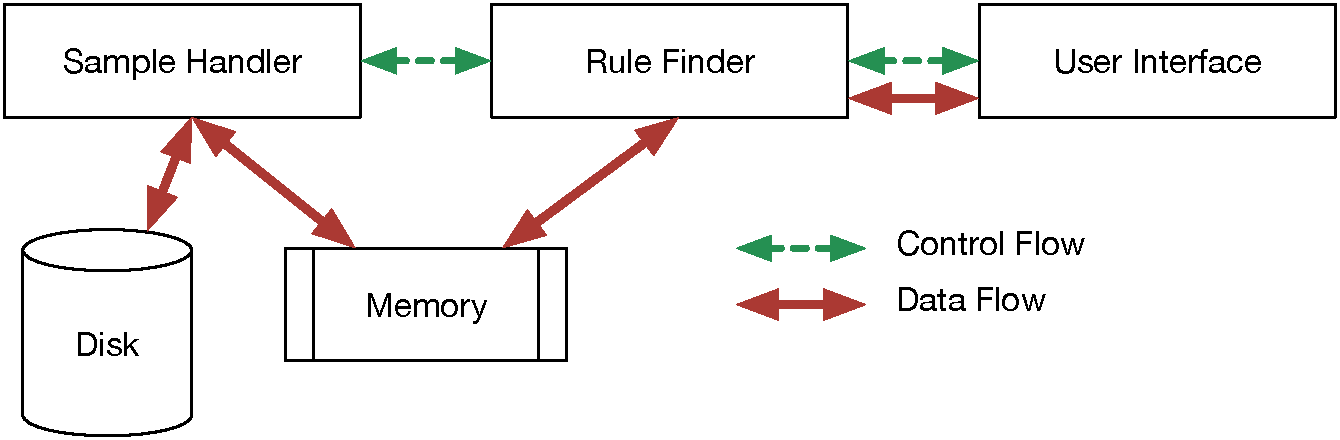
\includegraphics[width=80mm]{graphs/arch.pdf}
\vspace{-20pt}
\caption{The architecture our system \label{fig:system}}
\vspace{-15pt}
\end{figure}

Our system consists of three main components (shown in Figure~\ref{fig:system}): the `Rule Finder', the `Sample Handler' and the `User Interface'. 
At a high level, the User Interface is a web application that allows users to explore
a dataset using smart drill-down. The User Interface invokes the Rule Finder component based on interactions.
The Rule Finder determines what rules to display to a user based on the user's latest interaction, the values of parameters such as number $k$ of rules to display, weighting function $W$ to use, and so on. 
In order to do this, the Rule Finder has to make a pass through the table data several times. This can be expensive for big tables, so we dynamically maintain multiple samples of different parts of the table in memory instead. The Sample Handler is responsible for maintaining samples in memory and updating them when required. 
We now describe the components one by one.

\stitle{Rule Finder.} The problem addressed by the Rule Finder, i.e., that of choosing the optimal rule list of a given size, is NP-Hard. However, we find an approximately optimal solution as follows: We first notice that given a set of rules, a rule-list consisting of those rules has the highest score if the rules are sorted in decreasing order by weight. So we can define the score of a rule {\em set} to be the score of the rule-list obtained by ordering rules of the set in decreasing order by weight. Thus our problem reduces to that of finding the highest scoring rule set. As long as the weight function is monotonic, the score of a rule-set can be shown to be submodular. Then we use the fact that a submodular function can be optimized using a greedy algorithm to choose rules one at a time in a greedy manner until we have $k$ rules. We call the above algorithm BRS (which stands for {\bf B}est {\bf R}ule {\bf S}et). Additional details on our approximation algorithm can be found in our technical report~\cite{tr}. 

\stitle{Sample Handler.} The second component of our system, the `Sample Handler', takes two user-specified input parameters to begin with: the memory capacity $M$, and a parameter called $minSS$. $minSS$ determines the sample size required to run the BRS algorithm. Higher values of $minSS$ increase processing time (since the algorithm has to process a larger amount of data) but also increase the accuracy of the resulting displayed rule-list and rule counts. Then, the Sample Handler maintains a set of samples in memory, such that the sum of sizes of the samples never exceeds $M$. Each sample is a uniformly random subset of tuples that are covered by some rule $r'$. When the user attempts to drill-down on a rule $r$, the Sample Handler appropriately combines tuples from various existing samples to produce a set of at least $minSS$ tuples covered by $r$ to run BRS on. If the Sample Handler cannot create such a set using existing in-memory samples, then it needs to make a pass over the table to generate new samples. In that case, it determines a new set of samples to create, to maximize the probability that the next user click can be responded using those samples. Then it makes a pass through the table to create the new samples. 

%\begin{figure*}[ht]
%\vspace{-5pt}
%\centering
%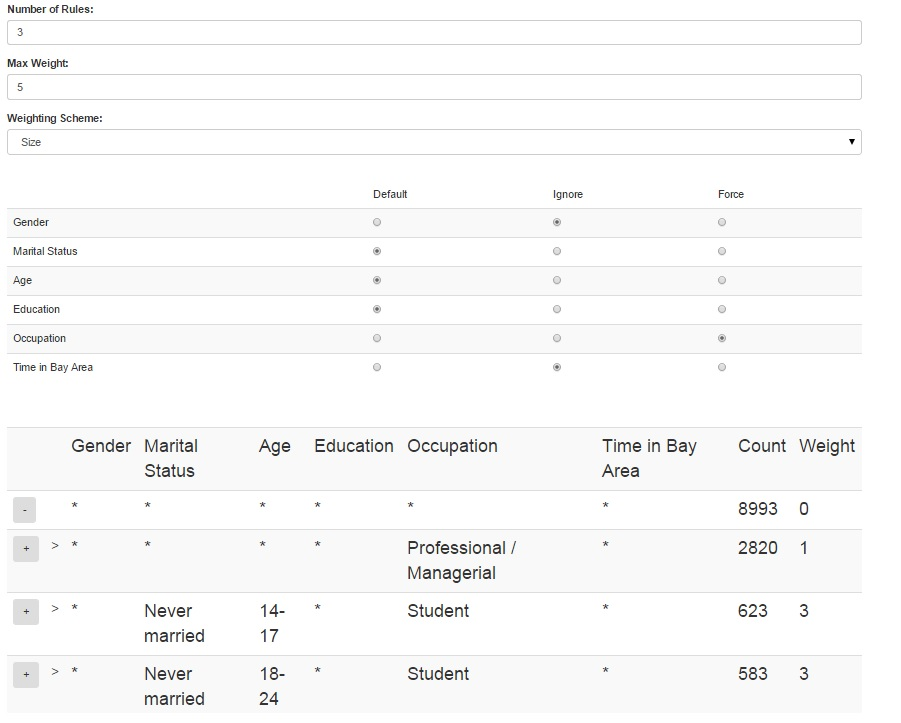
\includegraphics[width=160mm,frame]{graphs/tsapp_screenshot.jpg}
%\vspace{-5pt}
%\caption{The web interface of our system \label{fig:interface}}
%\vspace{-5pt}
%\end{figure*}

\begin{figure}[ht]
\vspace{-5pt}
\centering
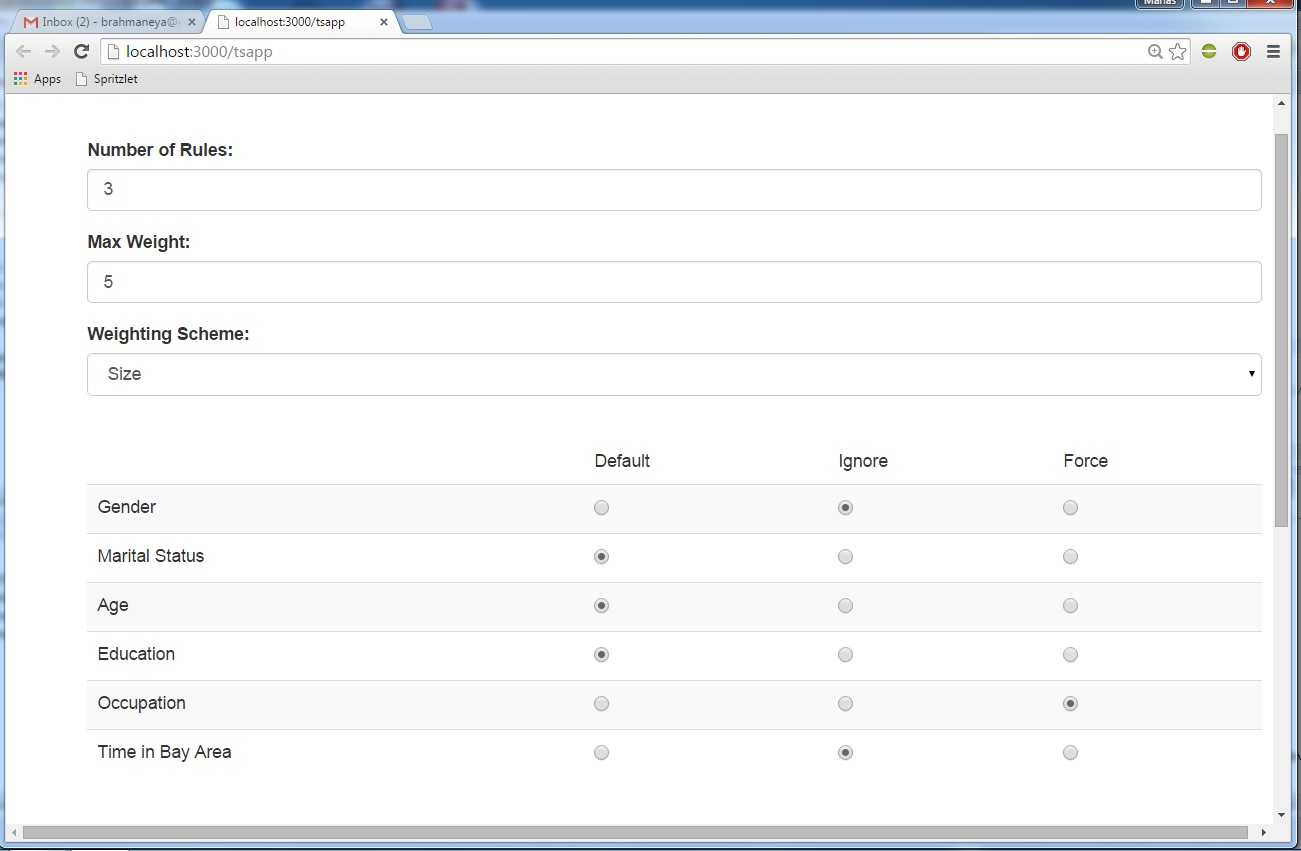
\includegraphics[width=80mm,frame]{graphs/uiscreenshot.jpg}
\vspace{-5pt}
\caption{The web interface of our system: specification of parameters \label{fig:interface}}
\vspace{-5pt}
\end{figure}

\begin{figure}[ht]
\vspace{-5pt}
\centering
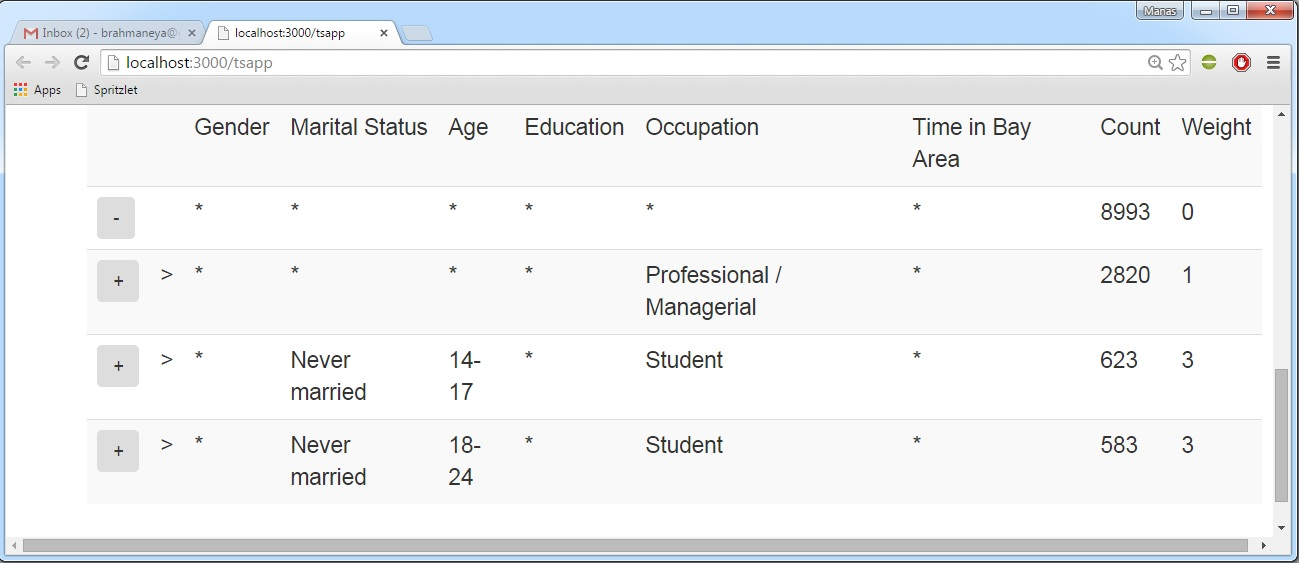
\includegraphics[width=80mm,frame]{graphs/uiresults.jpg}
\vspace{-5pt}
\caption{The web interface of our system: interactive results pane \label{fig:results}}
\vspace{-5pt}
\end{figure}

\stitle{User Interface.} The third component is the User Interface, 
shown in Figure~\ref{fig:interface}, with the results displayed in Figure~\ref{fig:results}.
At the top of the interface in Figure~\ref{fig:interface}, users can set the number 
of new rules to display in response to every smart drill-down. 

The second and third parameters manage weights, which as discussed in Section~\ref{sec:formal} allow a user to modify the interpretation of ``interesting tuples''.
The weighting function (set by the third parameter) is used to specify the importance of a rule, e.g., based on the number of distinct values or the value of particular attributes. In general, our approximation algorithm works for any monotonic weighting function. 
But for ease of use of the web interface, we have hard-coded a few different weighting functions, that can be selected using the drop-down list in the interface.

The second setting, a parameter called max weight, lets the system ignore rules that have high weight (above max weight). The idea behind this is that rules with high weight have a high number of non-$\star$ values, and hence a much smaller Count, making them unlikely to appear in an optimal rule-list. As max weight decreases, rule selection becomes more efficient. As long as the weight of all rules in the optimal rule-list is less than this
parameter, our system displays the optimal rule-list, so there is no impact on the user. However, if max weight is smaller than the weight of some optimal rules, then the user sees an non-optimal set of rules.

Below the drop down menu, the interface displays the set of columns of the database table being explored. Each column has three options: `Default', `Ignore', and `Force'. Choosing the Ignore option causes the column to be ignored, (so the weight given to a rule with a value in that column is set to that of a rule with a $\star$ value in that column). Choosing the Force option forces every displayed rule to have a non-$\star$ value in that column. This is especially useful for tables with a large number of columns, where the user may only be interested in some of the columns. 

Finally, the actual interactive table summary is displayed in Figure~\ref{fig:results}. The plus and minus buttons before the rules can be used to drill-down and reverse previous drill-downs. For instance, in the figure, the user has performed a single drill down using the Size weighting function (which sets weight to the number of non-star values of a rule), and choosing the Force option for the Occupation column, and Ignore for Gender and Time in Bay Area columns. As a result, the displayed rule-list (the three rules below the first one) all have a non-$\star$ value in the Occupation column, and only $\star$ values in the Gender and Time in Bay Area columns. Notice how the rules also have non-$\star$ values in some columns other than occupation, in contrast to traditional drill down.

%!TEX root = TableSummarizationDemo.tex
\vspace{-10pt}
\section{Demonstration Overview} \label{sec:demo} 
In our demonstration, we will show our prototype implementation of a system equipped with smart drill-down. We first describe the prototype implementation, the datasets, and then describe the demonstration scenarios.

\stitle{Prototype Details.} Our system is built as a web-application using NodeJS~\cite{nodejs}, with ExpressJS for the back-end, and AngularJS~\cite{angular} for the front-end. The Rule Finder and Sample Handler components (displayed in Figure~\ref{fig:system}) are coded in Java, and converted into an executable .jar that gets called by the web server backend. 

\stitle{Dataset Description.} In our demonstration, we will use two datasets. The first is an example of a dataset that attendees are not likely to be very familiar with, and the second is an example of a dataset that attendees are likely to be familiar with:

The first dataset, denoted `Marketing', contains demographic information about potential customers~\cite{dataset1}. A total of $9409$ questionnaires containing $502$ questions were filled out by shopping mall customers in the San Fransisco Bay Area; the dataset is a summary of their responses. Each tuple in the dataset describes a single person, with attributes such as gender, marital status, age, and so on. 

The second dataset is a US 1990 Census dataset from the UCI Machine Learning Repository~\cite{uciml}. It has 2.5 million tuples, with each tuple corresponding to a person. %In both the datasets, numerical columns such as age have been bucketized beforehand. 

\vspace{-1pt}
\stitle{Demonstration Scenarios.} The goal of demonstration is to (a) illustrate
the utility of smart drill-down, along with the various possible interactions, 
in comparison with traditional drill-down; 
(b) demonstrate the effect on performance and utility on varying parameters of the Rule Finder, as controlled by the user interface; here the attendees will select different settings and examine the response; and
(c) demonstrate the effect on performance and accuracy on varying sampling parameters of the Sample Handler, in-built in the system.   

During the demo, we will set up instances of the system with the two previously described datasets pre-loaded. We will also have the web user interface open in a browser window. Then for each demonstration, we will go though three scenarios one after the other:
\squishlist
\item {\bf Scenario 1: Comparison to drill-down}: We will start with some canned exploration scenarios to familiarize attendees with the system interface and its adjustable parameters. Through the scenarios, we will demonstrate how smart drill-down lets one quickly discover interesting information about a table, and how to tailor the table exploration to a user's interests. These scenarios will highlight the advantage of smart drill-down over traditional drill-down. 
\item {\bf Scenario 2: Rule Finder Parameters}: We will allow the attendees to vary parameters using the interface and observe their effects on the rules displayed, as well as response time and accuracy. Increasing the `Number of Rules' parameter will result in a longer rule list being displayed, but will cause an increase in response time. Reducing the `Max Weight' parameter, will speed up the response time of the system, but may result in a suboptimal rule-list being displayed. The third parameter, the weighting function, determines which rules the user finds `interesting'. Using a different weighting function, such as the `Bits' (which gives higher weight to rules containing non-$\star$ values in columns that have a large number of distinct values) will prioritize columns such as `Education' over columns such as `Gender' (since the latter has only two distinct values). The user will also be able to ignore certain columns, or force certain columns to be instantiated in the displayed rules. 
\item {\bf Scenario 3: Sample Handler Parameters}: We will allow attendees to try out multiple instances of the system initialized with different values of the $minSS$  parameter (recall that $minSS$ is the minimum sample size used by the system when determining which rules to display). This will allow attendees to observe how decreasing $minSS$ decreases running time but also potentially reduces accuracy of the displayed rules and their counts.
\squishend
\noindent With our demonstration, we hope to convince attendees that smart drill-down offers
a valuable alternative to traditional drill-down in quickly ``zooming into'' the interesting portions of a dataset.
%to add: summary of contributions (phrase as 'implemented' not as 'in this paper')
%overview of demo. what people will see in the demo. 

\balance

{\small
\bibliographystyle{abbrv}
\bibliography{TableSummarizationDemo}  
}

% Example of an appendix; typically would start on a new page
%pagebreak

\techreporttext{\input{appendix}}

\end{document}
